\documentclass[10pt,letterpaper,unboxed,cm]{article}
\usepackage{tgtermes} % times font
\usepackage{setspace}
%\doublespacing

\usepackage[margin=1in]{geometry}
\usepackage{graphicx}
\usepackage{amsmath}
\usepackage{amssymb}
\usepackage{xcolor}
\usepackage[export]{adjustbox}
\usepackage[linesnumbered,lined]{algorithm2e}
\usepackage{enumerate}
\usepackage[symbol]{footmisc}
\usepackage{textcomp}
\usepackage{dirtytalk}

\newcommand{\st}{~\mid~}
\newcommand{\ind}{$~~~$}
\newcommand{\todo}{\color{red} TODO: \color{black}}

\graphicspath{{images/}}

\renewcommand{\thefootnote}{\fnsymbol{footnote}}

\newcommand\blfootnote[1]{%
  \begingroup
  \renewcommand\thefootnote{}\footnote{#1}%
  \addtocounter{footnote}{-1}%
  \endgroup
}

\interfootnotelinepenalty=10000

\title{OpenOBD}

\date{June 10th, 2020}

\author{Cody Emrick\\A14740612 \and Christopher Madrigal\\A15702734}

\begin{document}

\maketitle

%\blfootnote{* From Special Collections}

\renewcommand*{\thefootnote}{\arabic{footnote}}

\tableofcontents
\newpage

\section{Abstract}

Vehicles seem to perpetually exist in a bygone era. By the time new cars adopt a technology, whether it be radio, CD players, or navigation systems, there's a very good chance that a similar feature has been available elsewhere for years beforehand. And when you want to upgrade, you will need to buy a new car to do so. Worst of all, you'll likely end up with a proprietary, custom solution with limited features. Shopping for a car based on the quality of the infotainment system is impractical, and even high-end cars are subject to this problem. Likewise, home mechanics that want access to diagnostic data will need to purchase a specialized, manufacturer-specific device just to read data. All vehicles since the mid-1990's come equipped with a standardized onboard diagnostic (OBD) system, but manufacturers and professional mechanics have done everything they can to lock consumers out of these vital systems. Our project proposes to break their monopoly on your car's data by allowing users and developers a safe, easy way to access and utilize data to enhance your vehicle's functionality and allow for modular upgrades.

\section{Introduction}

\subsection{The Problem}

Fundamentally, the core problem here is that most vehicles do not operate on a standard platform. Even similar models by the same manufacturer might only have a few parts in common, and even when a manufacturer creates a standardized platform, it's more for their benefit than the customer's and eventually they will do a refresh that will break compatibility. This forces aftermarket parts to be built around a specific make and model, perhaps with some flexibility based on the year or platform. Regardless, this has led to a quagmire of compatibility issues. For an aftermarket part manufacturer, there is little incentive to release an upgrade for a car nobody is buying new anymore. 

We can further sub-divide this problem into two classes: physical and electron. For example, if you want to buy a new radio for your car, you need to find one that both fits physically into your dashboard and also will connect to your car's audio system. On modern cars, your \say{infotainment} system may also contain many of the controls for your vehicle, or also display select diagnostic information, which means it must interface with whatever wiring and information specification the manufacturer provides. Our goal will be to tackle the latter issue, and we believe that, free of a requirement to match proprietary data connections, it will be easier to adapt a generic product to fit physically in a variety of vehicles. Even on modern vehicles with an Apple CarPlay or Android Auto are often difficult to upgrade and will not have access to a full range of information, although they are a step in the right direction.

Currently, the market is basically limited to infotainment systems. But we imagine that, with a unified platform to provide access to data, it might be possible to expand the market for other devices which can display data. It could be possible to project navigation and speedometer data directly onto your windshield, so you can keep your eyes on the road and also see where you are going. You could wear augmented reality glasses which highlight your car's location so you never get lost in a parking lot again. Your music player could change which playlist it's using based on your speed or location. You could be notified of an engine misfire when it happens. Your oil pressure could be read directly. You could use a machine learning algorithm to train yourself to drive more economically. We originally pitched ideas just like these, but kept running into the same issue: there is no standardized way to access your car's data for applications such as these, and if you developed a stack just for interfacing with the car then you could have to pick-and-choose which to use.

\subsection{The Goal}

We believe that someone looking to upgrade their vehicle should simply be able to go online or to a store, browse products that solve a problem they have, and then be able to use this in their car. They should not have to be locked-in to a given vendor or system, nor should they have to fear that they will lose access to their data or control of their car. As vehicles trend increasingly towards being \say{smart}, \say{Internet of Things} objects, the issues inherent in the modern smart-device ecosystem creep in to a traditionally very stable platform, and nobody should have to worry about their car being disabled or damaged remotely via exposure to a broader network. 

Additionally, as creators, we want more freedom to get data from our cars and to experiment with solutions to the problems with have. This is the basis of innovation, and currently any individual hoping to create a new product will have to navigate a technical minefield just to develop a one-off product for their own vehicle. A single man working alone ought to be able to create a solution and share this with others in whatever way they see fit. This is a fundamental aspect of \say{hacker culture}, and by lowering the bar to creating novel solutions we hope to spur innovation in this market.

Additionally, we think it's important that any third-party devices not have to compete over usage of the OBD-II port. By providing this as a modular part of a larger theoretical stack, free other devices to worry about doing their particular job correctly. 

\subsection{Our Solution}

However, all vehicles since the mid-1990's come equipped with the OBD-II specification for onboard diagnostics. This federally-mandated system provides a common interface for storing and accessing data relevant to your car's performance. Some manufacturers choose to build on top of this system to expand functionality.

With the above problems and goals in mind, we created the following guidelines for our device:

\begin{description}

\item [It Must Be Open:] In order for users to build on our work and audit its security, the platform must be open. A closed platform just adds one more inflexible, untrustworthy option.

\item [It Must Be Secure:] We want to authenticate communications between the user and their vehicle. While secrecy of the data is important, ensuring that requests come from and responses are returned to the owner of the vehicle and their authorized devices only is absolutely the most important thing. If the platform is insecure, it could leak private information about the user to malicious third-parties, or in a worst-case scenario, cause damage to their vehicle.

\item [It Must Be Safe:] The platform itself should reliably interface with vehicles without causing any harm. A developer should not be concerned that a bad write will brick their car's diagnostic computer. They must trust it to intercept and sanitize inputs to prevent mistaken or malicious commands.

\item [It Must Be Expandable:] The core set of OBD-II functions is standard across all vehicles, but we must allow for users to support additional functionality their manufacturer may provide. Additionally, users who want to write their own software or make their own hardware should be able to easily prototype on top of our platform.

With these goals in mind, we were able to take a common-sense approach to the design of our device, dubbed OpenOBD, which would allow us to interface easily with other devices while providing reliable service.

\end{description}

The Unix Philosophy is as follows:

\begin{enumerate}
  \item
  Write programs that do one thing and do it well.

  \item
  Write programs to work together.

  \item
  Write programs to handle text streams, because that is a universal interface.

\end{enumerate}

We wish to expand this philosophy into the domain of the Internet of Things.

\section{Technical Material}

\subsection{Prior Work}

\todo Examination of other products on the market and which of the above points they fail on.

\subsection{Design}

\begin{center}
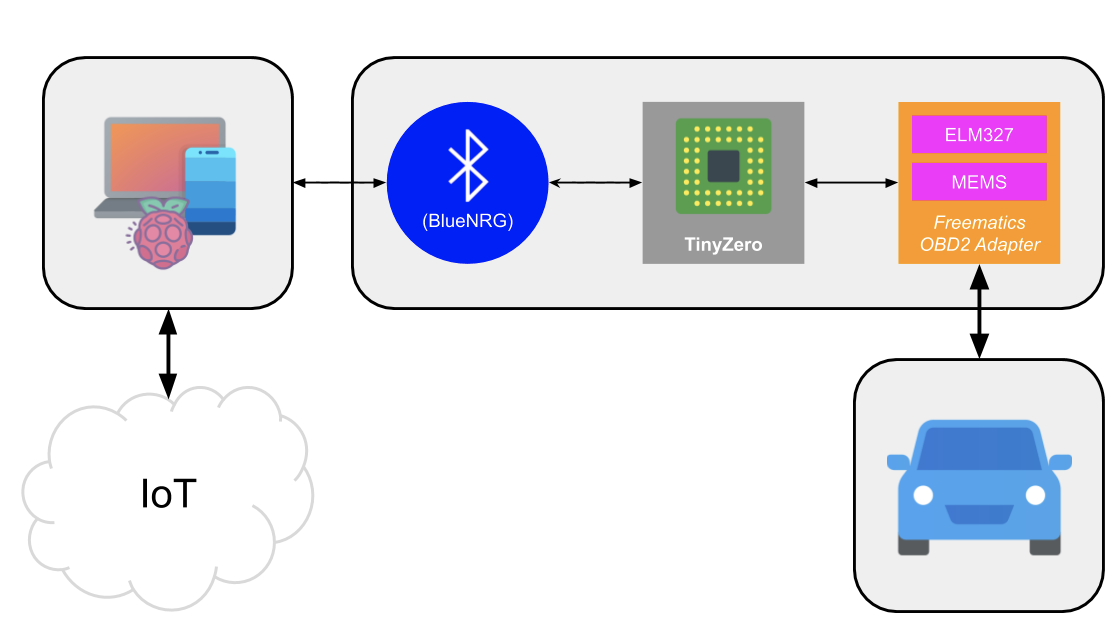
\includegraphics[width=0.7\linewidth]{pathway.png}
\end{center}

\todo High-level description of system.

\subsection{Platform}

For our Microcontroller, we selected the TinyZero by TinyCircuits. This is an ARM microcontroller that is modular and designed for prototyping. It is very small, which makes it ideal for prototyping a project that needs to fit into a compact package. The platform has excellent support for many embedded libraries, especially those designed for Arduino, and it supports a modular system of \say{stacking} modules, whereby a number of separate add-ons can simply be attached to each other, like a simplified Arduino HAT system. This makes it perfect for expanding functionality as we continue to prototype.

One decision we had to make was whether we implement our own OBD-II communicator. We ultimately chose not to do this for a variety of reasons. The OBD-II specification covers how data should be stored and transmitted, as well as what kind of data should be tracked and made available. A number of different, competing specifications for actually retrieving this data exist, and they vary greatly in voltage, pinout, and data format. This makes interpreting the data difficult and potentially hazardous to the vehicle if not done correctly. It would also have been more work than the rest of the project combined, and likely take up the majority of the time. Since commercial solutions for this connector exist, we decided it was better to focus on the novel aspects of our project and not to re-invent the wheel. After a survey of the market, we found two decent options, both of which use an ELM347 chip to handle the bulk of the work. After comparing options, a dongle by Freematics was cheaper and provided additional functionality built right in, so it became the obvious choice. Unfortunately, it did not arrive before the end of the quarter, likely due to shipping delays.

For communicating with other devices, we chose Bluetooth. It's the most common option for device-to-device connections, and modern Bluetooth with Low Energy (BLE) is quite efficient, which is important for a device which can potentially leech your car's battery. Ad-hoc Wi-Fi is just not efficient nor particularly secure, and interfacing over it would have been unnecessarily difficult for no additional advantages. It was important that consumer smartphones be able to interface directly with the OpenOBD module.

\newpage
\section{Milestones}

\begin{description}

\item [Read Data:] Physically read data from a device.
\item [Write Data:] Physically write data to the device.
\item [Expose Data:] Expose the data via an API
\item [Example Application:] Create a simple app that showcases how to use the API. Can also be used for debugging purposes.
\item [Encrypt Data:] Take this datapath and add user authentication.
\item [Allow Modifying Vehicle State:] Expose safe writes to the vehicle.
\item [Additional Sensors:] Add additional sensors to the device which cannot be found on many cars, such as GPS, accelerometer, etc.

\end{description}

\subsection{Read Data}

While we did not have a chance to test this (see the issues section below), we were able to use the ELM driver provided by Freematics for use with their dongle to implement wrappers which should read and write the data. The ELM utilizes UART to communicate with the microcontroller. A series of PIDs can be transmitted, and then a read will be performed via the OBD-II port. The result is then returned and passed to another wrapper to format a JSON response packet.

\subsection{Write Data}

Similar to Read Data, we could not test this, but we have implemented a dummy function in accordance with the documentation.

\subsection{Expose Data}

Our system is built around an API which processes and returns JSON structures. We expose the data by providing a clean, consistent specification for what fields to send and what sort of response to expect. Instead of having to know every PID that is implemented, you simply send a request for the fields you would like read and they, or an error, will be returned. This works, and while it is missing some of the expanded functionality of the Freematics dongle, the standard PIDs are all supported.

\subsection{Encrypt Data}

Upon activating the device, you will need to pair your device with it. This is done by generating an RSA keypair. The \say{public} key is then sent over (encrypted) Bluetooth to your device. This certificate can be shared to other devices you want to have access to your OpenOBD dongle. This provides authentication of the user/device. The Bluetooth spec itself provides encryption based around a PIN which the user must enter when it establishes a connection. This way, the data is encrypted and all identities can be verified. Since the device will automatically decrypt and encrypt with its private key, data sent elsewhere will be useless and requests from unauthorized users will likewise be invalid commands.

\subsection{Allow Modifying Vehicle State}

This is mostly unimplemented. While we have a specification for how to format a JSON write query, there is currently no wrapper to handle and format this data on the OpenOBD platform. The reason for this is that it is relatively low-priority. There are only a few writes you often want to do, such as clearing an error code, but writing is also the biggest source of vulnerabilities. Implementing a few simple writes would be possible, but it was decided to focus on other pathways and expand this later. Sanity-checking inputs is important.

\subsection{Additional Sensors}

We have added a GPS module and a storage module to our TinyZero. This allows tracking the vehicle's location remotely. We have plans to add a SIM Card module, to allow vehicle status to be tracked via the internet, but we do not have one of these modules. The Freematic UART dongle also allows for sensing battery levels, and we have implemented preliminary support for this, though it has gone untested. This and a few other optional PIDs exist as part of the ELM chip.

\section{Future Work}

\section{Conclusion}

\section{References}


%\footnote{\label{klooster}\textit{Revolutions in the Atlantic World}, Wim Klooster, 2018, New York Press}

\end{document}

